\documentclass[11pt]{article}

% Change to [preprint] for camera-ready draft without line numbers
\usepackage[review]{acl}

\usepackage{times}
\usepackage{latexsym}
\usepackage[T1]{fontenc}
\usepackage[utf8]{inputenc}
\usepackage{microtype}
\usepackage{inconsolata}
\usepackage{graphicx}
\usepackage{booktabs}
\usepackage{amsmath}
\usepackage{amssymb}
\usepackage{xcolor}
\usepackage{multirow}

\title{From Pixels to BFS: High Maze Accuracy\\Does Not Imply Visual Planning}

\author{Anonymous}

\usepackage{stfloats}

\makeatletter
\AtBeginDocument{\def\@maketitle{\vbox{\hsize\textwidth
 \linewidth\hsize \vskip 0.125in minus 0.125in \centering
 {\Large\bfseries \@title \par} \vskip 0.18in
 {\def\and{\unskip\enspace{\rmfamily and}\enspace}%
  \def\And{\end{tabular}\hss \egroup \hskip 1in plus 2fil
           \hbox to 0pt\bgroup\hss \begin{tabular}[t]{c}\bfseries}%
  \def\AND{\end{tabular}\hss\egroup \hfil\hfil\egroup
          \vskip 0.25in
           \hbox to \linewidth\bgroup\large \hfil\hfil
             \hbox to 0pt\bgroup\hss \begin{tabular}[t]{c}\bfseries}
  \hbox to \linewidth\bgroup\large \hfil\hfil
    \hbox to 0pt\bgroup\hss
  \outauthor
   \hss\egroup
    \hfil\hfil\egroup}
  \vskip 0.16in
  \begin{center}
    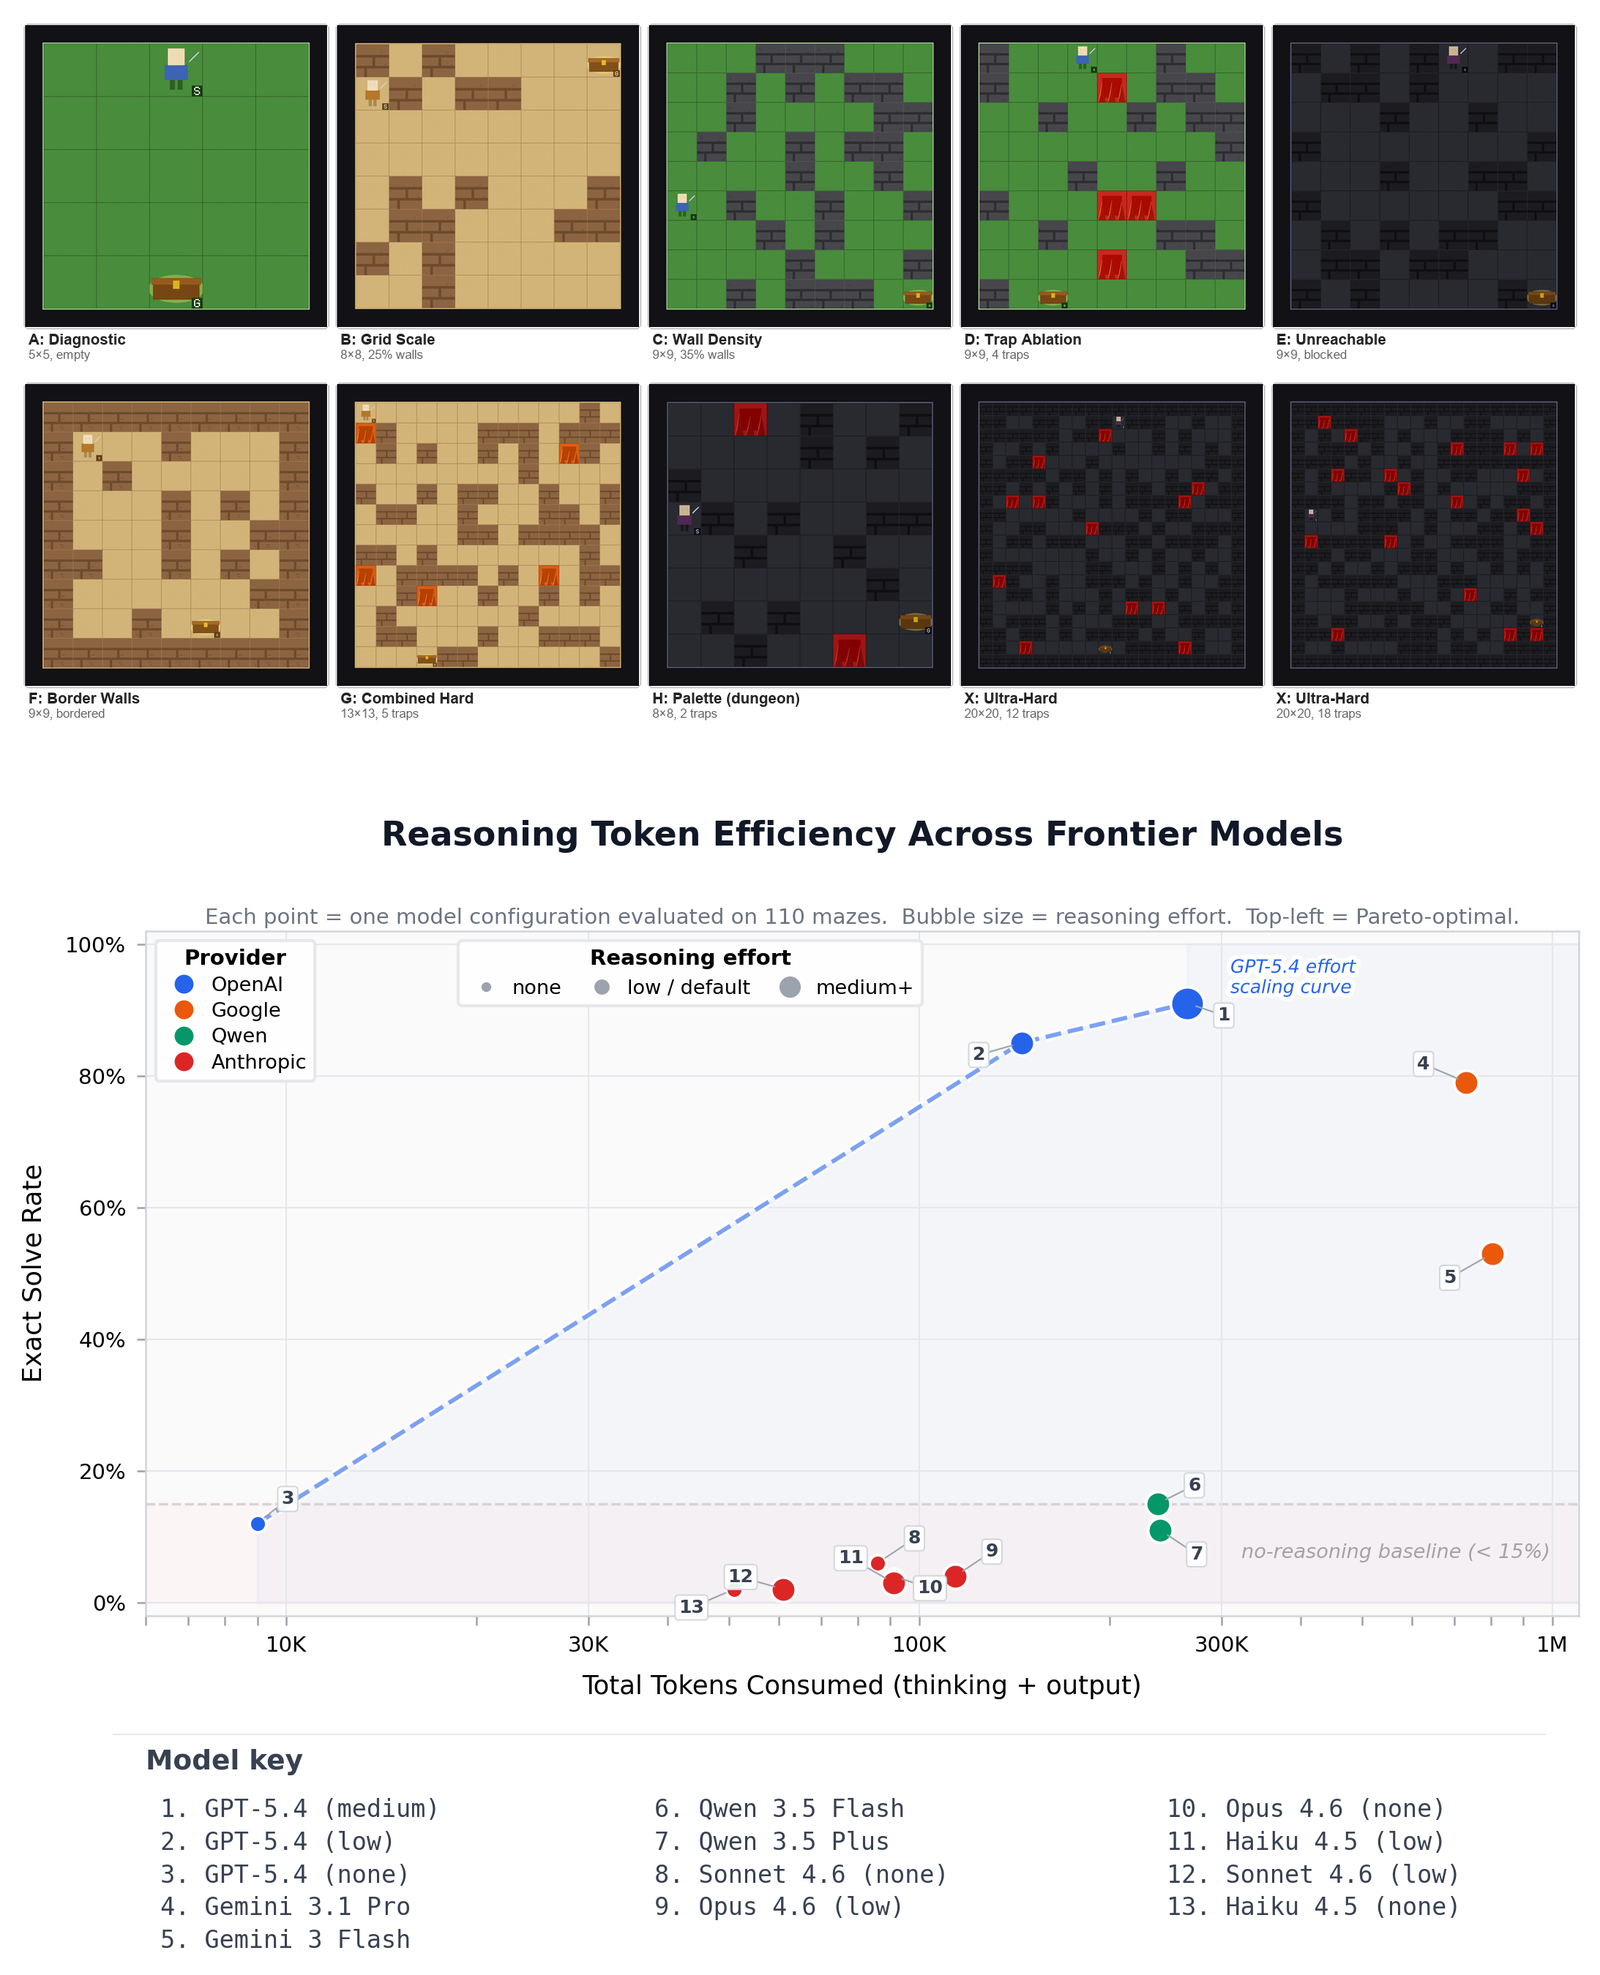
\includegraphics[width=0.96\textwidth]{fig_hero.png}
    \vspace{4pt}
    \parbox{\textwidth}{\fontsize{10pt}{12pt}\selectfont \textbf{Figure 1:} \textbf{Top:} Mazes from \textsc{MazeBench} at increasing difficulty: 5$\times$5 (A) to 20$\times$20 (X). \textbf{Bottom:} Solve rate vs.\ total tokens. Color = provider; size = reasoning effort. Claude (red) clusters at 2--6\%.}
  \end{center}
  \vskip 0.08in
}}}
\makeatother

\begin{document}
\maketitle
\setcounter{figure}{1}

% ==================================================================
%  ABSTRACT
% ==================================================================
\begin{abstract}
How do multimodal models solve visual spatial tasks---through genuine planning, or through brute-force search in token space?
We introduce \textsc{MazeBench}, a benchmark of 110 procedurally generated maze images across nine controlled groups, and evaluate 16 model configurations from OpenAI, Anthropic, Google, and Alibaba.
GPT-5.4 solves 91\% and Gemini~3.1~Pro 79\%, but these scores are misleading: models typically translate images into text grids and then enumerate paths step by step, consuming 1,710--22,818 tokens per solve for a task humans do quickly.
Without added reasoning budgets, all configurations score only 2--12\%; on 20$\times$20 ultra-hard mazes, they hit token limits and fail.
Qualitative traces reveal a common two-stage strategy: image-to-grid translation followed by token-level search, effectively BFS in prose.
A text-grid ablation shows Claude Sonnet~4.6 rising from 6\% on images to 80\% when given the correct grid, isolating weak visual extraction from downstream search.
When explicitly instructed not to construct a grid or perform graph search, models still revert to the same enumeration strategy.
\textsc{MazeBench} therefore shows that high accuracy on visual planning tasks does not imply human-like spatial understanding.
\end{abstract}

% ==================================================================
%  1  INTRODUCTION
% ==================================================================
\section{Introduction}

Multimodal large language models (MLLMs) have achieved impressive performance across a wide range of vision-language tasks, from visual question answering to diagram understanding and mathematical reasoning in visual contexts \cite{lu2024mathvista, yue2024mmmu, fu2024mme}.
Recent benchmarks have begun probing deeper visual capabilities, finding that models struggle with tasks that humans---even young children---solve effortlessly \cite{fu2024blink, tong2024eyes, chen2026babyvision}.
Yet when models \emph{do} score well on such tasks, a crucial question remains: \textbf{does a high accuracy score mean the model actually understands the task, or is it achieving the right answer through a fundamentally different---and far less efficient---mechanism?}

We investigate this question through visual maze solving, a task that is conceptually simple for humans: given a pixel-art maze image, find the shortest path from the player to the treasure.
A human glances at even a complex 20$\times$20 maze and traces the path visually in seconds.
We find that frontier MLLMs can also solve many of these mazes---GPT-5.4 achieves 91\%, Gemini~3.1~Pro 79\%---but they do so in a qualitatively different way.
Rather than spatial planning, models translate the image into a token-level grid representation and then perform \emph{serial path enumeration}: they brute-force the solution step by step in natural language, consuming thousands of reasoning tokens for a task that requires no deliberation for a human.
When the path is too long to enumerate within the token budget, the model gives up---not because it cannot see the maze, but because it runs out of space to think.

This finding has implications beyond mazes.
It suggests that benchmark accuracy alone can be misleading about the nature of model capabilities: a model may score 90\% on a task while using a fundamentally different---and far more costly---cognitive strategy than the one the benchmark was designed to measure.

We design \textsc{MazeBench} with three properties that make this analysis possible:

\paragraph{Controlled difficulty via procedural generation.}
We build a procedural maze generator producing mazes with controlled grid size (5$\times$5 to 20$\times$20), wall density (0--55\%), trap count (0--25), border walls, and varied start/goal positions.
Ground-truth shortest paths are computed via BFS.
The 110 mazes are organized into nine experimental groups---including diagnostic, grid scale, wall density, trap ablation, and ultra-hard---enabling clean ablation studies (Figure~1).

\paragraph{Reasoning effort as a controlled variable.}
We systematically vary the reasoning budget via frontier API controls (OpenAI's \texttt{reasoning\_effort}, Anthropic's adaptive thinking), producing a scaling curve from no thinking to medium effort on the \emph{same} visual inputs.

\paragraph{Token efficiency as a window into strategy.}
We report the total tokens consumed (thinking + output) per solve.
This reveals \emph{how} models solve mazes, not just whether they do: GPT-5.4~low requires 1,710 tokens per solve, while Gemini~3~Flash uses 15,171---both achieving correct answers but through vastly different amounts of brute-force enumeration (Figure~1).

Our main findings are:

\begin{enumerate}
\itemsep0em
\item \textbf{High scores mask brute-force strategies.} GPT-5.4 solves 91\% of mazes, but consumes 2,913 tokens per solve---serial enumeration, with no observable spatial planning behavior. On 20$\times$20 mazes where paths exceed the token budget, accuracy drops to 30\% (Section~\ref{sec:ultrahard}).

\item \textbf{Without added reasoning budgets, performance remains very low.} All 16 configurations score only 2--12\% in their no-thinking or lowest-budget settings, even when some parse the grid correctly. For the stronger models, the failure is primarily in path planning rather than basic visual parsing (Section~\ref{sec:diagnostic}).

\item \textbf{The same task, radically different costs.} Models vary by 9$\times$ in tokens per solve (1,710 for GPT-5.4 vs.\ 15,171 for Gemini~3~Flash), revealing that ``solving a maze'' means very different things computationally across providers (Section~\ref{sec:efficiency}).

\item \textbf{Model size does not buy spatial reasoning.} Claude Opus~4.6 (the largest Anthropic model) solves the same 4\% as Haiku~4.5 (the smallest). Spatial planning does not appear to be an emergent property of scale (Section~\ref{sec:analysis}).
\end{enumerate}

% ==================================================================
%  2  RELATED WORK
% ==================================================================
\section{Related Work}

\paragraph{Visual perception gaps in MLLMs.}
Several recent benchmarks have documented systematic failures in visual perception.
BLINK \cite{fu2024blink} reformats 14 classic computer vision tasks as multiple-choice questions and finds that GPT-4V achieves only 51\% versus 96\% for humans, concluding that perception tasks ``resist mediation through natural language.''
\citet{tong2024eyes} identify ``CLIP-blind pairs''---images that vision encoders conflate despite clear visual differences---and construct the MMVP benchmark exposing failures on basic visual patterns.
BabyVision \cite{chen2026babyvision} tests core visual abilities that human children master by age 3--6, finding that even Gemini~3~Pro scores only 49.7 versus 94.1 for adults.
Notably, BabyVision includes a maze-tracing task in which models select which entrance connects to an exit from a multiple-choice list---a \emph{perceptual tracking} task.
Our benchmark differs fundamentally: rather than choosing among predefined options, models must \emph{generate} the complete shortest path as an exact sequence of moves (U/D/L/R), requiring both visual parsing and multi-step spatial planning.
This distinction allows us to show that failures compound across \emph{both} stages: some models (Claude) fail primarily at visual grid extraction, while others (GPT-5.4, Gemini) parse the grid correctly but still resort to brute-force token enumeration rather than spatial planning.

\paragraph{Multimodal reasoning benchmarks.}
MathVista \cite{lu2024mathvista} and MathVerse \cite{zhang2024mathverse} evaluate mathematical reasoning in visual contexts, finding that models often rely on textual cues rather than diagram understanding.
EMMA \cite{hao2025emma} tests cross-modal reasoning across math, physics, chemistry, and coding, reporting that even chain-of-thought prompting and test-time compute scaling underperform (ICML~2025).
MMMU \cite{yue2024mmmu} and MME \cite{fu2024mme} provide comprehensive evaluation suites spanning dozens of disciplines, while MMEvalPro \cite{huang2025mmevalpro} addresses systematic biases in multiple-choice evaluation by introducing perception prerequisite questions.
\citet{chen2024right} audit evaluation methodology itself, questioning whether current benchmarks measure the capabilities they claim to.
Our benchmark complements this body of work by targeting a single, tightly controlled task---visual pathfinding---that isolates spatial reasoning from domain knowledge.

\paragraph{Spatial reasoning in MLLMs.}
Spatial reasoning has emerged as a key evaluation axis for multimodal models.
SpatialVLM \cite{chen2024spatialvlm} endows VLMs with metric spatial reasoning via synthetic data, while SpatialRGPT \cite{cheng2024spatialrgpt} grounds spatial reasoning in depth-aware representations.
SpatialBench \cite{xu2025spatialbench} decomposes spatial intelligence into five cognitive levels and finds that models fail at high-level planning.
SpatiaLab \cite{tong2026spatialab} evaluates spatial reasoning in unconstrained real-world images, finding that even GPT-5-mini scores only 41\% versus 65\% for humans.
GSR-Bench \cite{rajabi2024gsrbench} evaluates grounded spatial relationship understanding across 27~models at NeurIPS~2024.
VGRP-Bench \cite{ren2025vgrpbench} is the most directly related benchmark to ours, testing vision-language models on grid-based visual reasoning puzzles.
Our work differs in three ways: (1)~we introduce reasoning effort as a controlled experimental variable, (2)~we report thinking token efficiency as a metric, and (3)~we demonstrate through qualitative analysis that models solve grid puzzles through brute-force token-level enumeration, with no evidence of human-like spatial planning.

\paragraph{Test-time compute scaling.}
\citet{snell2025scaling} demonstrate that scaling inference-time computation can be more effective than scaling model parameters for reasoning tasks (ICLR~2025).
\citet{liu2025art} show that no single test-time scaling strategy universally dominates but that performance scales monotonically with compute budget.
Chain-of-Visual-Thought \cite{chen2025covt} and related methods \cite{chen2025mcot} extend chain-of-thought reasoning to continuous visual tokens.
Our reasoning effort sweep provides direct empirical evidence for these theoretical results: GPT-5.4 improves from 12\% to 85\% to 91\% as reasoning effort increases from none to low to medium, with diminishing returns at higher budgets.

% ==================================================================
%  3  BENCHMARK DESIGN
% ==================================================================

\section{Benchmark Design}
\label{sec:benchmark}

\subsection{Task Formulation}

Given a pixel-art maze image, the model must return a JSON object containing: the grid size, whether the start and goal are found, whether a path exists (\texttt{reachable}), the shortest path length, and the exact path as a list of directional moves (\texttt{U}, \texttt{D}, \texttt{L}, \texttt{R}).
A maze is scored as \emph{solved} only when all three conditions hold: (1)~reachability is correctly identified, (2)~the shortest path length is correct, and (3)~the returned path exactly matches one of the accepted shortest-path annotations.
No partial credit is awarded.

\subsection{Procedural Maze Generation}

We build a procedural generator that produces mazes with controlled parameters.
Each maze is defined by a grid size ($r \times c$), wall density $d \in [0, 0.55]$ (fraction of candidate cells converted to walls), trap count $t$ (impassable hazard tiles visually distinct from walls), and optional border walls (a wall ring around the outer edge).
Start and goal positions are randomized on opposite edges with a minimum Manhattan distance of $\lfloor(r+c)/3\rfloor$.

The generation algorithm places walls incrementally, verifying after each placement that the maze remains reachable (unless the maze is designated unreachable).
Traps are placed similarly with reachability checks.
Ground-truth shortest paths are computed via breadth-first search with multi-parent tracking, enumerating all optimal paths (capped at 50).
All mazes render as $1024 \times 1024$ pixel PNG images using procedurally generated pixel-art sprites across four visual palettes (forest, desert, dungeon, meadow).

\subsection{Dataset Structure}

The benchmark contains 110 mazes organized into nine groups:

\begin{itemize}
\itemsep0em
\item \textbf{Group~A: Diagnostic} (8 mazes). Empty or near-empty grids with straight-line paths. If a model fails here, the bottleneck is visual parsing, not reasoning.
\item \textbf{Group~B: Grid Scale} (15). Constant wall density (25\%), grid sizes from $5 \times 5$ to $13 \times 13$. Isolates the effect of spatial scale.
\item \textbf{Group~C: Wall Density} (15). Constant $9 \times 9$ grid, density swept from 0\% to 45\%. Isolates obstacle complexity.
\item \textbf{Group~D: Trap Ablation} (12). Six matched pairs sharing the same random seed---one with traps, one without---isolating trap recognition.
\item \textbf{Group~E: Unreachable} (14). All unreachable, spanning $5 \times 5$ to $13 \times 13$. Tests false-positive rate for reachability claims.
\item \textbf{Group~F: Border Walls} (10). Five matched pairs with/without border walls. Tests whether visual framing affects parsing.
\item \textbf{Group~G: Combined Hard} (16). Large grids ($9 \times 9$--$13 \times 13$), high density, traps, and borders combined.
\item \textbf{Group~H: Palette Stress} (10). Same maze structure rendered in all four palettes. Tests visual style sensitivity.
\item \textbf{Group~X: Ultra-Hard} (10). $20 \times 20$ grids with 8--25 traps, 35--55\% wall density, and shortest paths of 28--42 steps.
\end{itemize}

Overall the dataset contains 79 reachable mazes (72\% of the 110) and 31 unreachable (28\%).
Shortest path lengths range from 4 to 42 moves (mean 13.5, median 12).

% ==================================================================
%  4  EXPERIMENTAL SETUP
% ==================================================================

\section{Experimental Setup}
\label{sec:setup}

\paragraph{Models.}
We evaluate models from four providers:
\textbf{OpenAI}: GPT-5.4 and GPT-5.4-mini, each at three reasoning effort levels (none, low, medium);
\textbf{Anthropic}: Claude Opus~4.6, Sonnet~4.6, and Haiku~4.5, each at no-thinking and low-effort configurations;
\textbf{Google}: Gemini~3.1~Pro~Preview and Gemini~3~Flash~Preview;
\textbf{Alibaba/Qwen}: Qwen~3.5~Plus and Qwen~3.5~Flash via DashScope.
This yields 16 model configurations in total.

\paragraph{Protocol.}
Every configuration receives the same fixed prompt instructing JSON-only output with no tool use.
Images are sent as base64-encoded data URLs.
We disable structured output enforcement and tool calling across all APIs so that models must reason freely.
Failed JSON parses are retried up to twice.

\paragraph{Reasoning effort control.}
For OpenAI, we use the \texttt{reasoning\_effort} parameter (none/low/medium).
For Anthropic, we test both no-thinking (omitting the thinking configuration) and adaptive thinking with low effort.
We do not evaluate Claude at higher reasoning budgets because the text-grid ablation (Section~\ref{sec:textgrid}) establishes that Claude's failure is in visual extraction, not downstream search---additional reasoning tokens applied to a misidentified grid yield no improvement and would not constitute a controlled comparison.
Gemini and Qwen models use default configurations; notably, Gemini performs hidden internal reasoning (visible via \texttt{thoughtsTokenCount} in the API response) that cannot be disabled.

\paragraph{Reproducibility.}
All experiments were conducted between March~20--23, 2026 using the following API model identifiers: \texttt{gpt-5.4} and \texttt{gpt-5.4-mini} (OpenAI Responses API), \texttt{claude-opus-4-6}, \texttt{claude-sonnet-4-6}, and \texttt{claude-haiku-4-5-20251001} (Anthropic Messages API, version \texttt{2023-06-01}), \texttt{gemini-3.1-pro-preview} and \texttt{gemini-3-flash-preview} (Gemini REST API), and \texttt{qwen3.5-plus} and \texttt{qwen3.5-flash} (DashScope API).
Temperature was set to 0.0 for all non-thinking configurations; Anthropic requires temperature~1.0 when thinking is enabled.

% ==================================================================
%  5  RESULTS
% ==================================================================

\section{Results}
\label{sec:results}

\subsection{Main Results}

Table~\ref{tab:leaderboard} presents the full leaderboard ranked by solve rate on the 100-maze core set (excluding Group~X ultra-hard).

\begin{table}[t]
\centering
\small
\begin{tabular}{@{}lrrr@{}}
\toprule
\textbf{Model} & \textbf{Solved} & \textbf{Reach.\%} & \textbf{Lat.(s)} \\
\midrule
GPT-5.4 (medium) & 91/100 & 95 & 38.1 \\
GPT-5.4 (low) & 85/100 & 92 & 23.8 \\
Gemini 3.1 Pro & 79/100 & 86 & 51.9 \\
Gemini 3 Flash & 53/100 & 82 & 32.3 \\
GPT-5.4-mini (medium) & 51/100 & 86 & 21.8 \\
GPT-5.4-mini (low) & 49/100 & 89 & 7.3 \\
Qwen 3.5 Flash & 15/100 & 71 & 12.2 \\
GPT-5.4 (none) & 12/100 & 71 & 2.1 \\
Qwen 3.5 Plus & 11/100 & 78 & 23.7 \\
GPT-5.4-mini (none) & 8/100 & 79 & 1.3 \\
Sonnet 4.6 (none) & 6/100 & 70 & 16.9 \\
Opus 4.6 (low) & 4/100 & 67 & 21.3 \\
Opus 4.6 (none) & 4/100 & 71 & 19.8 \\
Haiku 4.5 (low) & 3/100 & 63 & 9.1 \\
Sonnet 4.6 (low) & 2/100 & 60 & 14.7 \\
Haiku 4.5 (none) & 2/100 & 68 & 9.4 \\
\bottomrule
\end{tabular}
\caption{Main leaderboard on the 100-maze core set. \textbf{Solved} requires correct reachability, correct shortest path length, and exact path match. \textbf{Reach.\%} is reachability accuracy. \textbf{Lat.} is average latency per maze.}
\label{tab:leaderboard}
\end{table}

The results reveal a clear hierarchy.
GPT-5.4 with medium reasoning dominates at 91\%, followed by GPT-5.4~low (85\%) and Gemini~3.1~Pro (79\%).
All Claude models score between 2--6\% regardless of model size (Haiku, Sonnet, Opus) or thinking configuration.
Notably, enabling low-effort thinking on Claude models does not improve---and sometimes degrades---performance (Sonnet drops from 6\% to 2\%).

\subsection{Reasoning Effort Scaling}
\label{sec:scaling}

Table~\ref{tab:scaling} presents per-group solve counts across all 16 model configurations, revealing both the effect of reasoning effort and stark cross-provider differences.

\begin{table*}[t]
\centering
\small
\begin{tabular}{@{}ll rrrrrrrr r@{}}
\toprule
& & \multicolumn{8}{c}{\textbf{Solves per Group}} & \\
\cmidrule(lr){3-10}
\textbf{Model} & \textbf{Reason.} & \textbf{A} & \textbf{B} & \textbf{C} & \textbf{D} & \textbf{E} & \textbf{F} & \textbf{G} & \textbf{H} & \textbf{Total} \\
& & \tiny{/8} & \tiny{/15} & \tiny{/15} & \tiny{/12} & \tiny{/14} & \tiny{/10} & \tiny{/16} & \tiny{/10} & \tiny{/100} \\
\midrule
GPT-5.4          & med.    & 7 & 14 & 13 & 12 & 13 & 9 & 13 & 10 & \textbf{91} \\
GPT-5.4          & low     & 8 & 13 & 10 & 11 & 12 & 8 & 13 & 10 & \textbf{85} \\
GPT-5.4          & none    & 8 &  1 &  1 &  1 &  1 & 0 &  0 &  0 & 12 \\
GPT-5.4-mini     & med.    & 7 & 11 &  8 &  6 &  7 & 3 &  5 &  4 & 51 \\
GPT-5.4-mini     & low     & 6 &  9 &  8 &  5 & 11 & 3 &  3 &  4 & 49 \\
GPT-5.4-mini     & none    & 5 &  0 &  0 &  1 &  2 & 0 &  0 &  0 &  8 \\
\midrule
Gemini 3.1 Pro   & default & 8 & 12 & 14 &  9 &  9 & 7 & 10 & 10 & \textbf{79} \\
Gemini 3 Flash   & default & 7 &  7 &  9 &  7 &  6 & 5 &  7 &  5 & \textbf{53} \\
\midrule
Qwen 3.5 Flash   & default & 8 &  1 &  2 &  1 &  2 & 0 &  1 &  0 & 15 \\
Qwen 3.5 Plus    & default & 6 &  1 &  4 &  0 &  0 & 0 &  0 &  0 & 11 \\
\midrule
Sonnet 4.6       & none    & 3 &  0 &  1 &  1 &  0 & 0 &  0 &  1 &  6 \\
Sonnet 4.6       & low     & 1 &  0 &  1 &  0 &  0 & 0 &  0 &  0 &  2 \\
Opus 4.6         & none    & 2 &  0 &  1 &  0 &  1 & 0 &  0 &  0 &  4 \\
Opus 4.6         & low     & 2 &  0 &  1 &  0 &  1 & 0 &  0 &  0 &  4 \\
Haiku 4.5        & none    & 1 &  1 &  0 &  0 &  0 & 0 &  0 &  0 &  2 \\
Haiku 4.5        & low     & 3 &  0 &  0 &  0 &  0 & 0 &  0 &  0 &  3 \\
\bottomrule
\end{tabular}
\caption{Per-group solve counts for all 16 model configurations. Groups: \textbf{A}=Diagnostic, \textbf{B}=Grid Scale, \textbf{C}=Wall Density, \textbf{D}=Trap Ablation, \textbf{E}=Unreachable, \textbf{F}=Border Walls, \textbf{G}=Combined Hard, \textbf{H}=Palette Stress. GPT-5.4's none$\to$low transition (+73 solves) is the largest single improvement. All Claude models remain at 2--6 regardless of reasoning effort. Gemini models achieve strong results via hidden internal thinking.}
\label{tab:scaling}
\end{table*}

For GPT-5.4, the transition from no reasoning to low effort produces a dramatic +73 solve improvement (12$\to$85), while increasing to medium adds only +6 (85$\to$91), exhibiting clear diminishing returns.
The hard group (G) plateaus at 13/16 at both low and medium, suggesting that the remaining failures require qualitatively different capabilities rather than more reasoning tokens.

In contrast, all Claude models remain flat at 2--6 solves regardless of reasoning configuration---Sonnet actually \emph{degrades} from 6 to 2 with low effort enabled.
Gemini models, which perform hidden reasoning by default, achieve results between GPT-5.4's low and medium configurations without any user-controllable effort setting.
Qwen models show modest performance (11--15), with the smaller Flash variant slightly outperforming Plus---the only family where the smaller model does better.

\subsection{Diagnostic Analysis: Vision Works, Reasoning Doesn't}
\label{sec:diagnostic}

Group~A (diagnostic) serves as a critical control.
These eight mazes have zero or near-zero walls with straight-line paths---any model that can parse the grid should solve them.
GPT-5.4 achieves 8/8 \emph{even without reasoning}, confirming that its vision encoder correctly identifies the grid, start position, goal position, and tile types.
GPT-5.4's collapse from 8/8 on diagnostics to 1/15 on Group~B (which adds only 25\% wall density) demonstrates that the failure is entirely in path planning, not visual parsing.

Interestingly, Claude models struggle even on diagnostics: Opus solves only 2/8 and Haiku 1/8 without thinking.
This suggests that Claude's vision pipeline has additional limitations in grid parsing that compound with the reasoning deficit.

\subsection{Unreachable Detection}

Unreachable mazes probe a different failure mode: can models recognize when no path exists?
Without reasoning, all models exhibit a strong bias toward claiming reachability---GPT-5.4 produces 25/28 false positives (89\% false-positive rate).
With medium reasoning, this drops to 6/28 (21\%), and unreachable detection reaches 93\% recall.
This suggests that detecting impossibility is itself a reasoning-intensive task: the model must exhaustively verify that no path exists rather than optimistically reporting one.

\subsection{Thinking Token Efficiency}
\label{sec:efficiency}

Figure~1 and Table~\ref{tab:efficiency} report total tokens consumed (thinking + output) per solve, revealing order-of-magnitude differences in reasoning efficiency.

\begin{table}[t]
\centering
\small
\begin{tabular}{@{}lrrr@{}}
\toprule
\textbf{Model} & \textbf{Solved} & \textbf{Tot.~Tok.} & \textbf{Tok/Solve} \\
\midrule
GPT-5.4 (medium) & 91 & 265K & 2,913 \\
GPT-5.4 (low) & 85 & 145K & 1,710 \\
Gemini 3.1 Pro & 79 & 731K & 9,250 \\
Gemini 3 Flash & 53 & 804K & 15,171 \\
GPT-5.4-mini (medium) & 51 & 503K & 9,872 \\
GPT-5.4-mini (low) & 49 & 152K & 3,105 \\
Qwen 3.5 Flash & 15 & 238K & 15,835 \\
GPT-5.4 (none) & 12 & 9K & 782 \\
Qwen 3.5 Plus & 11 & 240K & 21,804 \\
GPT-5.4-mini (none) & 8 & 11K & 1,427 \\
Opus 4.6 (none) & 4 & 91K & 22,818 \\
\bottomrule
\end{tabular}
\caption{Thinking token efficiency. \textbf{Tot.~Tok.} is total thinking + output tokens across all 100 mazes. \textbf{Tok/Solve} is the average total tokens consumed per correctly solved maze. Lower is more efficient.}
\label{tab:efficiency}
\end{table}

GPT-5.4 at low effort is the Pareto-optimal configuration: 85 solves at 1,710 tokens per solve.
Medium effort buys 6 more solves at a 70\% token cost increase.
Gemini~3~Flash consumes 7,186 thinking tokens per maze internally (visible via the API's \texttt{thoughtsTokenCount} field) but achieves only 53\% solve rate---5.5$\times$ more total tokens than GPT-5.4~low for 38\% fewer solves.
Claude models are the least efficient, spending 22,000--30,000 tokens per solve on verbose but incorrect outputs.

A key revelation is that Gemini models perform hidden reasoning by default: Gemini~3~Flash uses a median of 7,861 thinking tokens per maze despite having no user-configurable reasoning toggle.
The Gemini--Claude gap, however, is not solely explained by thinking tokens.
As our qualitative analysis in Section~\ref{sec:analysis} shows, Claude models produce inaccurate grid extractions (wrong dimensions, misplaced walls), meaning they brute-force on a \emph{hallucinated} grid---a compounding failure where poor vision quality renders even extensive reasoning futile.

\subsection{Ultra-Hard Ceiling}
\label{sec:ultrahard}

Group~X ($20 \times 20$ grids, 8--25 traps, paths of 28--42 steps) tests the absolute ceiling of current models.
Table~\ref{tab:ultrahard} shows per-maze results for GPT-5.4 at medium effort---the best-performing configuration on the core set.

\begin{table}[t]
\centering
\small
\begin{tabular}{@{}lccrcr@{}}
\toprule
\textbf{Maze} & \textbf{GT} & \textbf{Pred.} & \textbf{Path} & \textbf{Solved} & \textbf{Lat.} \\
\midrule
101 & \checkmark & \checkmark & 40 $\to$ 18 & & 88s \\
102 & \checkmark & \checkmark & 30 $\to$ 30 & \checkmark & 89s \\
103 & \checkmark & $\times$ & 42 $\to$ -- & & 148s \\
104 & $\times$ & $\times$ & -- & $\triangle$ & 123s \\
105 & \checkmark & \checkmark & 32 $\to$ 32 & \checkmark & 85s \\
106 & \checkmark & $\times$ & 37 $\to$ -- & & 134s \\
107 & $\times$ & $\times$ & -- & \checkmark & 108s \\
108 & \checkmark & $\times$ & 28 $\to$ -- & & 137s \\
109 & \checkmark & $\times$ & 41 $\to$ -- & & 124s \\
110 & $\times$ & $\times$ & -- & $\triangle$ & 130s \\
\midrule
\multicolumn{4}{@{}l}{Total solved} & \textbf{3/10} & 117s \\
\bottomrule
\end{tabular}
\caption{GPT-5.4 (medium) on the 10 ultra-hard 20$\times$20 mazes. \textbf{GT} = ground-truth reachability; \textbf{Pred.} = model prediction; \textbf{Path} = GT length $\to$ predicted length. \checkmark = correct, $\times$ = wrong, $\triangle$ = correct reachability but incomplete output (hit token limit). The model solves only the two shortest reachable paths (30, 32 steps) and falsely declares all paths $\geq$37 unreachable.}
\label{tab:ultrahard}
\end{table}

GPT-5.4 drops from 91\% on the core set to \textbf{3/10} on ultra-hard.
Average latency increases to 117 seconds (versus 38s on the core set), and 5/10 mazes hit the maximum output token limit (8,192 tokens).
Of the 7 reachable ultra-hard mazes, the model falsely declares 4 unreachable---it runs out of reasoning budget before finding the path and defaults to reporting no solution.
The two mazes it does solve have paths of 30 and 32 steps (the shorter end of the ultra-hard range), while all paths $\geq$37 steps are missed.

This provides direct evidence that models solve mazes through serial enumeration bounded by token budget: when the path exceeds what can be brute-forced within the thinking allocation, the model fails.

% ==================================================================
%  6  ANALYSIS AND DISCUSSION
% ==================================================================

\section{Analysis and Discussion}
\label{sec:analysis}

\paragraph{A universal two-stage strategy.}
Examination of model outputs reveals that \emph{all} models---regardless of provider or accuracy---follow the same two-stage strategy:
\textbf{(1)~Image-to-grid translation}: the model converts the visual maze into a textual row-column matrix, and
\textbf{(2)~Serial path enumeration}: the model attempts to trace paths step-by-step through this textual grid.
What differentiates high-performing models from low-performing ones is primarily the quality of Stage~1, not the sophistication of Stage~2.

Claude models expose this strategy clearly because their reasoning traces are visible in the output.
On \texttt{gen\_maze\_014} (an 8$\times$8 grid), Opus~4.6 outputs a full grid transcription before searching:

\vspace{2pt}
{\small\ttfamily
\noindent Row 0: W, open, W, W, open, open, ...G\\
Row 1: W, S, open, W, W, W, open, ...\\
\mbox{[...maps all 10 rows...]}\\
Path: R,R,R,...(1,3) wait, (1,3) is wall.\\
Alternative: (1,1)→(1,2)→(2,2)→(2,3)→...\\
That's: R, D, R, R, R, R, R, R, R, U, U = 11\\
Shorter: ... = 11 moves. Or: ... = 15, longer.\\
Stick with 11.}
\vspace{2pt}

This is textbook brute-force search in natural language: try a path, hit a wall, backtrack, try another, count steps, compare.
Notably, our prompt explicitly instructs models not to ``use any external tools, code, search, calculators, or graph-search programs''---yet the models' only available strategy is to \emph{simulate} a graph-search algorithm (BFS) in natural language tokens, step by step.
Critically, both Opus and Sonnet \textbf{misidentify the grid as 10$\times$10} (it is actually 8$\times$8), leading them to reason over a hallucinated grid and produce incorrect paths.
GPT-5.4 correctly identifies 8$\times$8 and Gemini~3~Flash also reports the correct grid size---their Stage~1 is more accurate, which makes their Stage~2 brute-force search succeed on the correct grid.

\paragraph{The performance gap is in vision, not reasoning strategy.}
This two-stage analysis reframes the cross-provider performance differences.
Claude models do not fail because they use a worse \emph{reasoning} strategy---they use the same enumerate-and-backtrack approach as GPT-5.4.
They fail because their \emph{grid extraction} is unreliable: wrong grid dimensions, mislocated walls, and hallucinated openings.
On the trivially empty diagnostic maze \texttt{gen\_maze\_001} (5$\times$5, zero walls), Sonnet~4.6 reports a ``6$\times$6 grid'' instead of the correct 5$\times$5 and computes a path of length~4---the correct length, but from a misidentified grid.
Opus~4.6 reports ``7$\times$7'' and returns a path of length~5, both incorrect (the grid is 5$\times$5 with shortest path~4).

On the unreachable maze \texttt{gen\_maze\_057}, this vision deficit is catastrophic: Opus maps a 9$\times$9 grid as 11$\times$11 with incorrectly placed walls, then brute-forces a 14-step path \emph{through cells that are actually walls}---confidently declaring the maze reachable when it is not.
GPT-5.4 without reasoning correctly reports this maze as unreachable in 2.6 seconds, demonstrating superior visual parsing even without any chain-of-thought.

\paragraph{High accuracy still means brute-force.}
The crucial insight is that even the best-performing models---GPT-5.4 at 91\%, Gemini~3.1~Pro at 79\%---are still brute-forcing.
They simply brute-force on a \emph{correct} grid.
The evidence is threefold:
(1)~Performance scales with thinking token budget, not with any spatial heuristic---adding more tokens yields more solves, in a pattern consistent with longer serial search.
(2)~On ultra-hard 20$\times$20 mazes, GPT-5.4 hits the token limit and gives up, declaring 4/7 reachable mazes ``unreachable.''
A human traces the same maze visually in seconds.
(3)~Token efficiency varies by 9$\times$ across providers (1,710 vs.\ 15,171 tokens per solve), consistent with different search strategies expressed in text but inconsistent with human-like spatial planning, which should not require proportionally more computation for the same visual structure.

This is fundamentally different from human maze solving.
Humans engage spatial perception directly---tracing paths with their eyes, recognizing dead ends holistically, and planning routes without step-by-step enumeration.
Models convert vision to language, then search through language.
The conversion step is lossy (especially for Claude), and the search step is computationally expensive relative to the task's intrinsic difficulty.

\paragraph{Can prompting induce visual reasoning?}
A natural question is whether the brute-force strategy is a prompt artifact---perhaps the standard prompt implicitly encourages grid-based reasoning.
We test this with a modified ``visual-intuition'' prompt that explicitly instructs: \emph{``Do NOT convert the maze into a text grid, matrix, or row/column representation. Do NOT perform step-by-step BFS, DFS, or any graph-search algorithm in text. Instead, solve this the way a human would: look at the image, visually trace the walkable path.''}

On 20 representative mazes, GPT-5.4 (low) scores 17/20 with the visual prompt versus 19/20 with the standard prompt---slightly \emph{worse}, not better.
More revealing is what happens when we apply the visual prompt to Claude Sonnet~4.6, whose reasoning traces are visible.
Despite the explicit prohibition, Sonnet immediately falls back to grid enumeration:

\vspace{2pt}
{\small\ttfamily
\noindent Let me map out the walls (brown brick tiles)\\
and open paths (tan/sand tiles):\\
Row 0 (top): walls at col 0, col 2, then open\\
from col 3-8, wall at col 8-9 area\\
Row 1: Start at col 1, wall at col 1-2 area,\\
wall at col 3-5 area, open right side\\
\mbox{[...continues mapping all rows...]}}
\vspace{2pt}

In this setting, the model does not comply with the instruction to reason visually.
Instead, it falls back to converting the image into a textual grid representation and then enumerating paths through it---exactly the brute-force strategy the prompt forbids.
Crucially, the model never acknowledges this limitation---it silently violates the constraint rather than reporting that it cannot solve the task under the given restrictions.
This raises a broader concern about instruction compliance: when a model lacks the capability to follow a constraint, it proceeds with a forbidden strategy rather than failing gracefully.

\paragraph{Text-grid ablation confirms vision is the bottleneck.}
To directly test whether Claude's failure is in vision or reasoning, we bypass the image encoder entirely: we provide Sonnet~4.6 with the \emph{correct text grid} (using \texttt{S}, \texttt{G}, \texttt{.}, \texttt{\#}, \texttt{T} symbols) instead of the maze image.
Table~\ref{tab:textgrid} shows the results.

\begin{table}[t]
\centering
\small
\begin{tabular}{@{}lrrr@{}}
\toprule
\textbf{Input} & \textbf{Solved} & \textbf{Tok/Solve} & \textbf{Lat.} \\
\midrule
Image (none)    &  6/100 & 14,313 & 16.9s \\
Text grid (low) & 80/100 &  3,222 & 34.8s \\
\bottomrule
\end{tabular}
\caption{Sonnet~4.6: image vs.\ text grid on 100 mazes. Bypassing vision yields 13$\times$ more solves and 4.4$\times$ better token efficiency.}
\label{tab:textgrid}
\end{table}

With low-effort reasoning on the text grid, Sonnet solves \textbf{80/100} mazes---a 13$\times$ improvement over image input (6/100).
This places text-grid Sonnet between GPT-5.4~low (85/100) and Gemini~3.1~Pro (79/100)---models that rank among the best with image input.
Token efficiency also improves dramatically: 3,222 tokens per solve with text input versus 14,313 with images---a 4.4$\times$ gain.
With images, Sonnet produces 86K output tokens but solves only 6~mazes (verbose, incorrect reasoning on hallucinated grids); with text, it produces 258K tokens but solves 80~mazes (productive reasoning on correct input).

This confirms that Claude's reasoning engine is competitive with the best models when given accurate spatial input.
The bottleneck is entirely in the image-to-grid translation stage---the same brute-force search that fails on a hallucinated grid succeeds on the correct one.
\label{sec:textgrid}

\paragraph{Model size does not buy spatial reasoning.}
Claude Opus~4.6 solves only 4/100---fewer than GPT-5.4 with no reasoning (12/100), and comparable to Haiku~4.5.
This is consistent with Claude's documented gap on MMMU \cite{yue2024mmmu} (80.7\% vs.\ GPT-5's 85.4\% and Gemini~3~Pro's 81.0\%).

\paragraph{Hidden reasoning explains the Gemini advantage.}
Gemini outperforms Claude (53--79\% vs.\ 2--6\%) because it performs hidden reasoning by default: Gemini~3~Flash uses a median of 7,861 thinking tokens per maze, while Claude reports zero.
Combined with more accurate grid extraction, this enables effective brute-force search on correct grids.

% ==================================================================
%  7  CONCLUSION
% ==================================================================

\section{Conclusion}
\label{sec:conclusion}

We introduced \textsc{MazeBench}, a benchmark of 110 procedurally generated visual mazes that probes not just \emph{whether} multimodal models can solve spatial tasks, but \emph{how} they do so.

Our main message is simple: \textbf{high accuracy on visual planning tasks can be misleading}.
The strongest models in our benchmark do solve many mazes, but they do not appear to solve them the way humans do.
Instead, they first translate pixels into a textual grid and then search for a path in token space, step by step.
This strategy is computationally expensive, brittle under scale, and qualitatively different from rapid visual path tracing.

This distinction matters for evaluation.
GPT-5.4 reaches 91\% on the 100-maze core set, yet still relies on serial token-level search and collapses on ultra-hard mazes when the search no longer fits within the token budget.
Claude models expose the same search strategy even more clearly, but often on incorrect grid extractions; when we replace the image with the correct text grid, Sonnet jumps from 6\% to 80\%, showing that weak performance can come from poor visual extraction while strong performance can still come from brute-force planning.

Taken together, our results suggest that benchmark scores should not be read as evidence of human-like spatial understanding.
They are evidence only that a model can eventually produce the correct answer under a particular compute budget.
To measure genuine multimodal progress, we need evaluations that track not just correctness, but also \emph{strategy}, \emph{efficiency}, and failure mode.

\section*{Limitations and Future Work}

The benchmark uses procedurally generated pixel-art mazes and proprietary API-based models, and cross-provider reasoning controls are not perfectly comparable; future work should extend the setup to open models, human timing baselines, and broader visual planning domains.

% ==================================================================
%  REFERENCES
% ==================================================================
\bibliography{references}

\clearpage
\appendix
\onecolumn

\section{Complete Maze Dataset by Group}
\label{app:mazes}

Figures~\ref{fig:app_a}--\ref{fig:app_x} show every maze in the benchmark organized by experimental group.

\begin{figure}[ht]
\centering
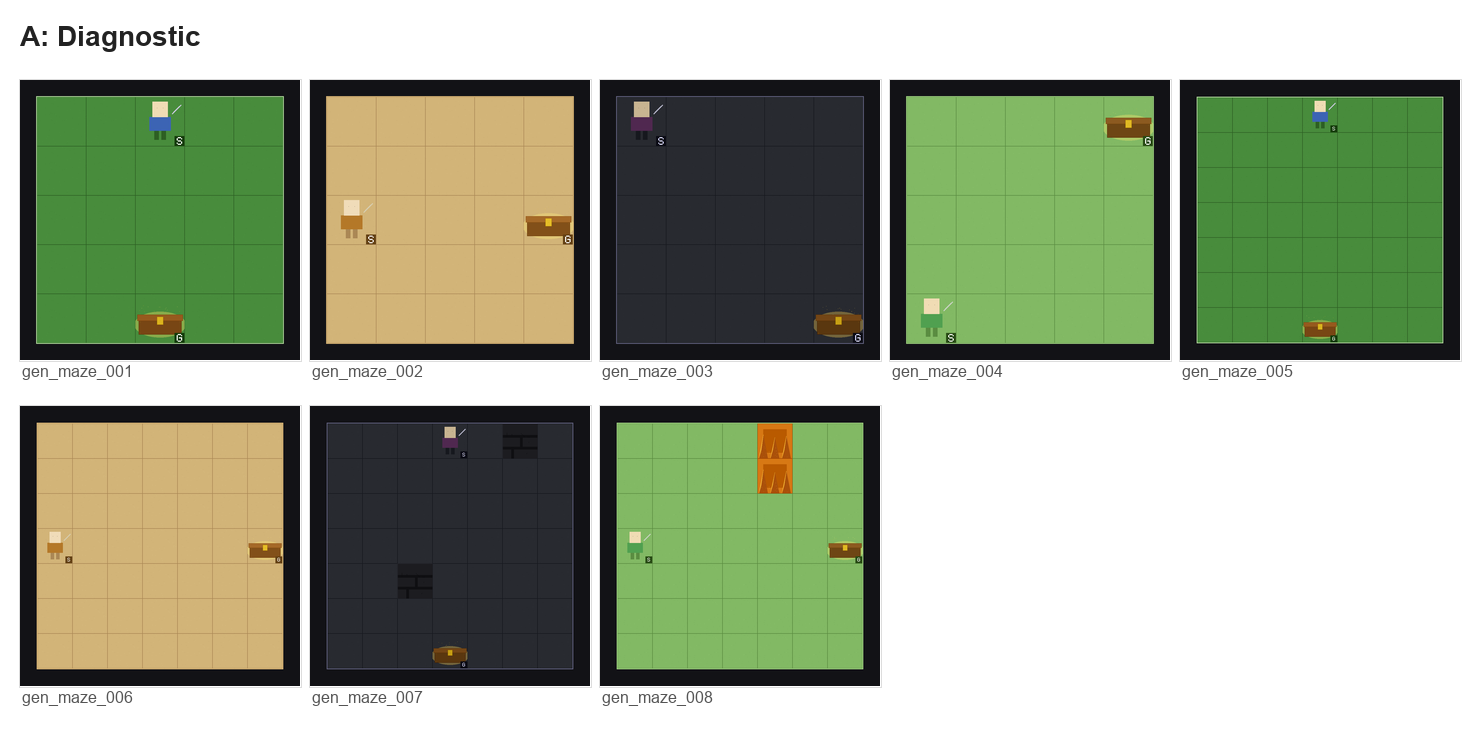
\includegraphics[width=0.85\textwidth]{appendix_group_a.png}
\caption{Group~A: Diagnostic (8 mazes). Empty or near-empty grids with trivial straight-line paths.}
\label{fig:app_a}
\end{figure}

\begin{figure}[ht]
\centering
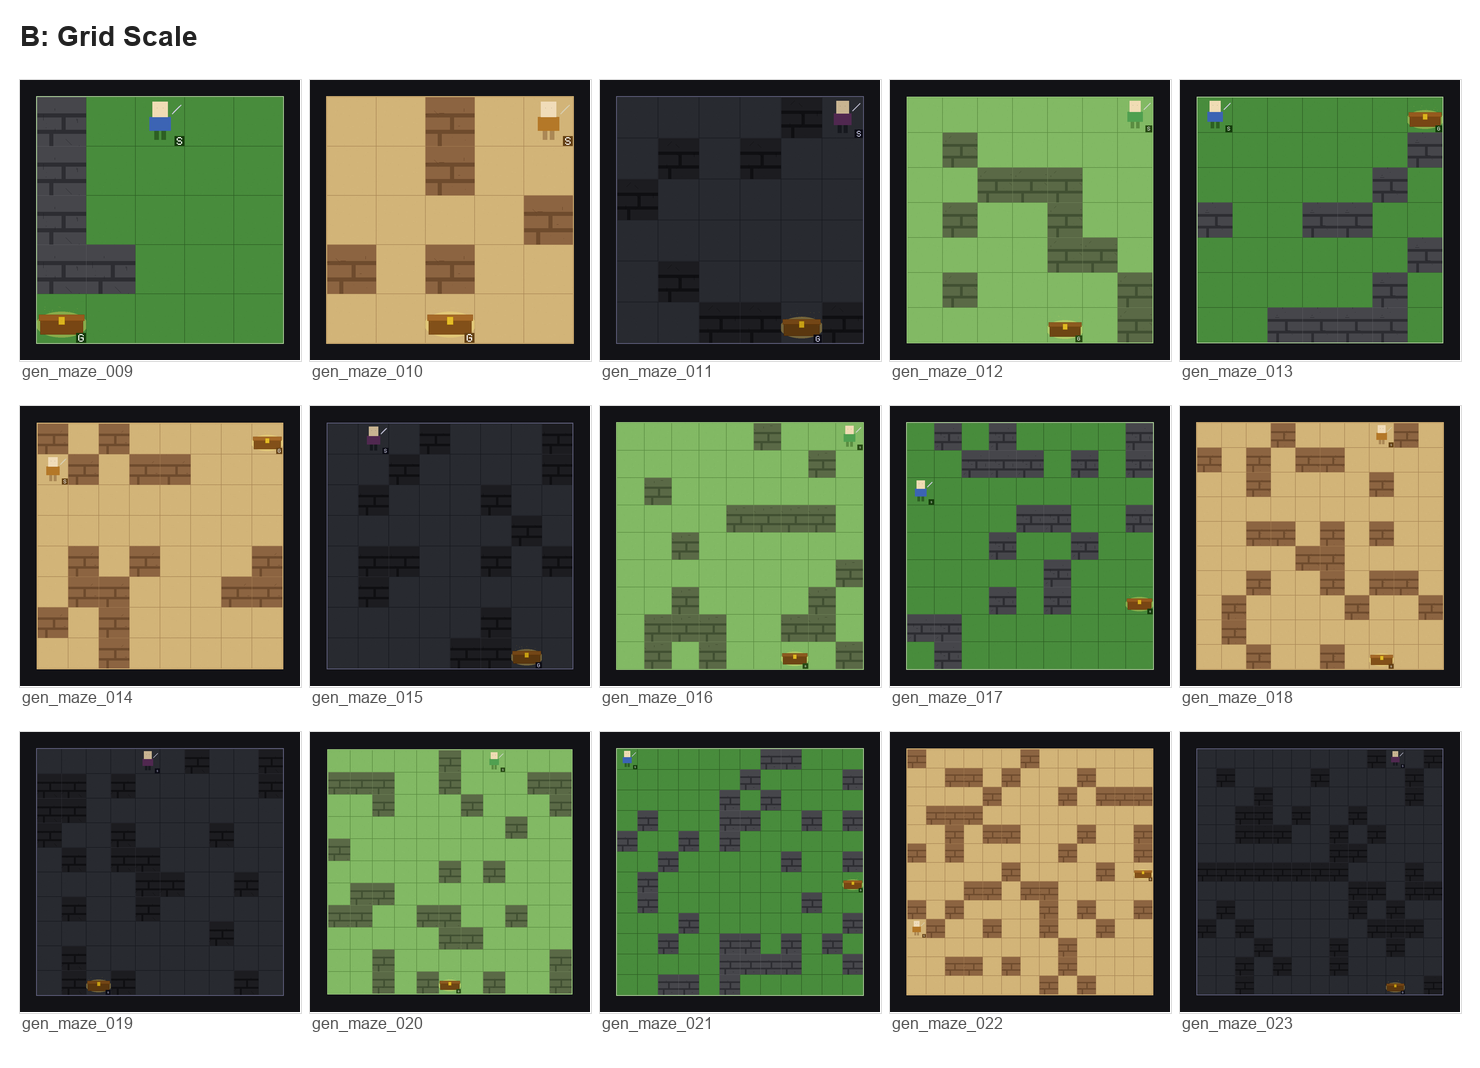
\includegraphics[width=0.85\textwidth]{appendix_group_b.png}
\caption{Group~B: Grid Scale (15 mazes). Constant 25\% wall density, grid sizes from $5 \times 5$ to $13 \times 13$.}
\label{fig:app_b}
\end{figure}

\begin{figure}[ht]
\centering
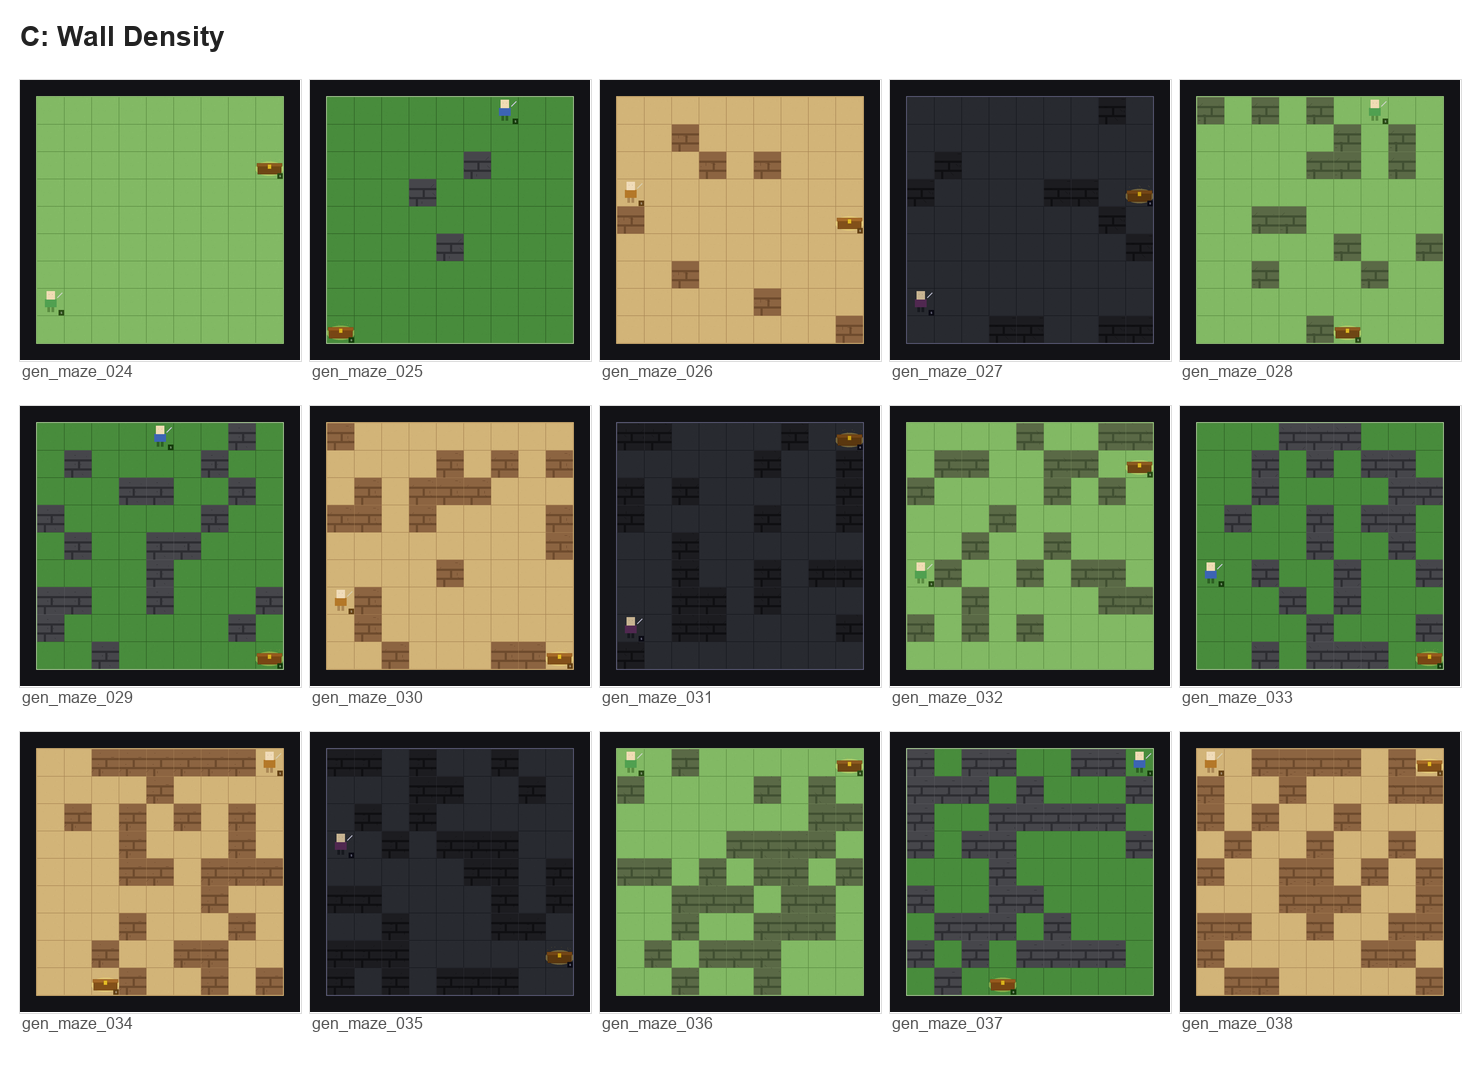
\includegraphics[width=0.85\textwidth]{appendix_group_c.png}
\caption{Group~C: Wall Density (15 mazes). Constant $9 \times 9$ grid, density from 0\% to 45\%.}
\label{fig:app_c}
\end{figure}

\begin{figure}[ht]
\centering
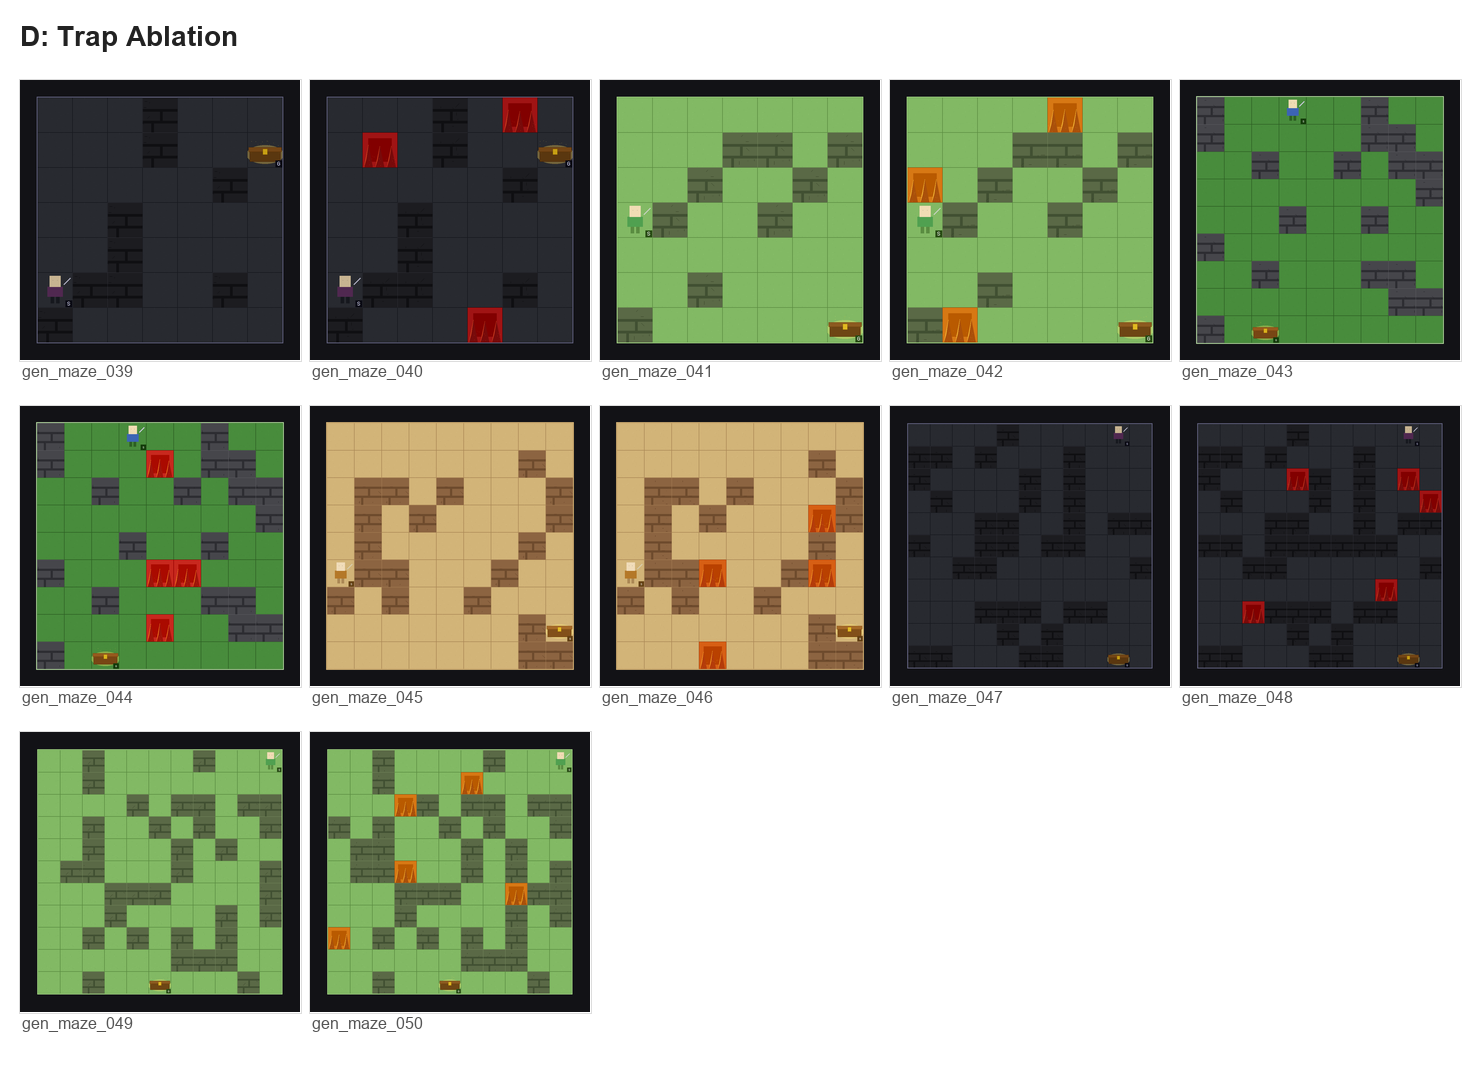
\includegraphics[width=0.85\textwidth]{appendix_group_d.png}
\caption{Group~D: Trap Ablation (12 mazes). Six matched pairs---control (no traps) and treatment (with traps)---sharing the same random seed.}
\label{fig:app_d}
\end{figure}

\begin{figure}[ht]
\centering
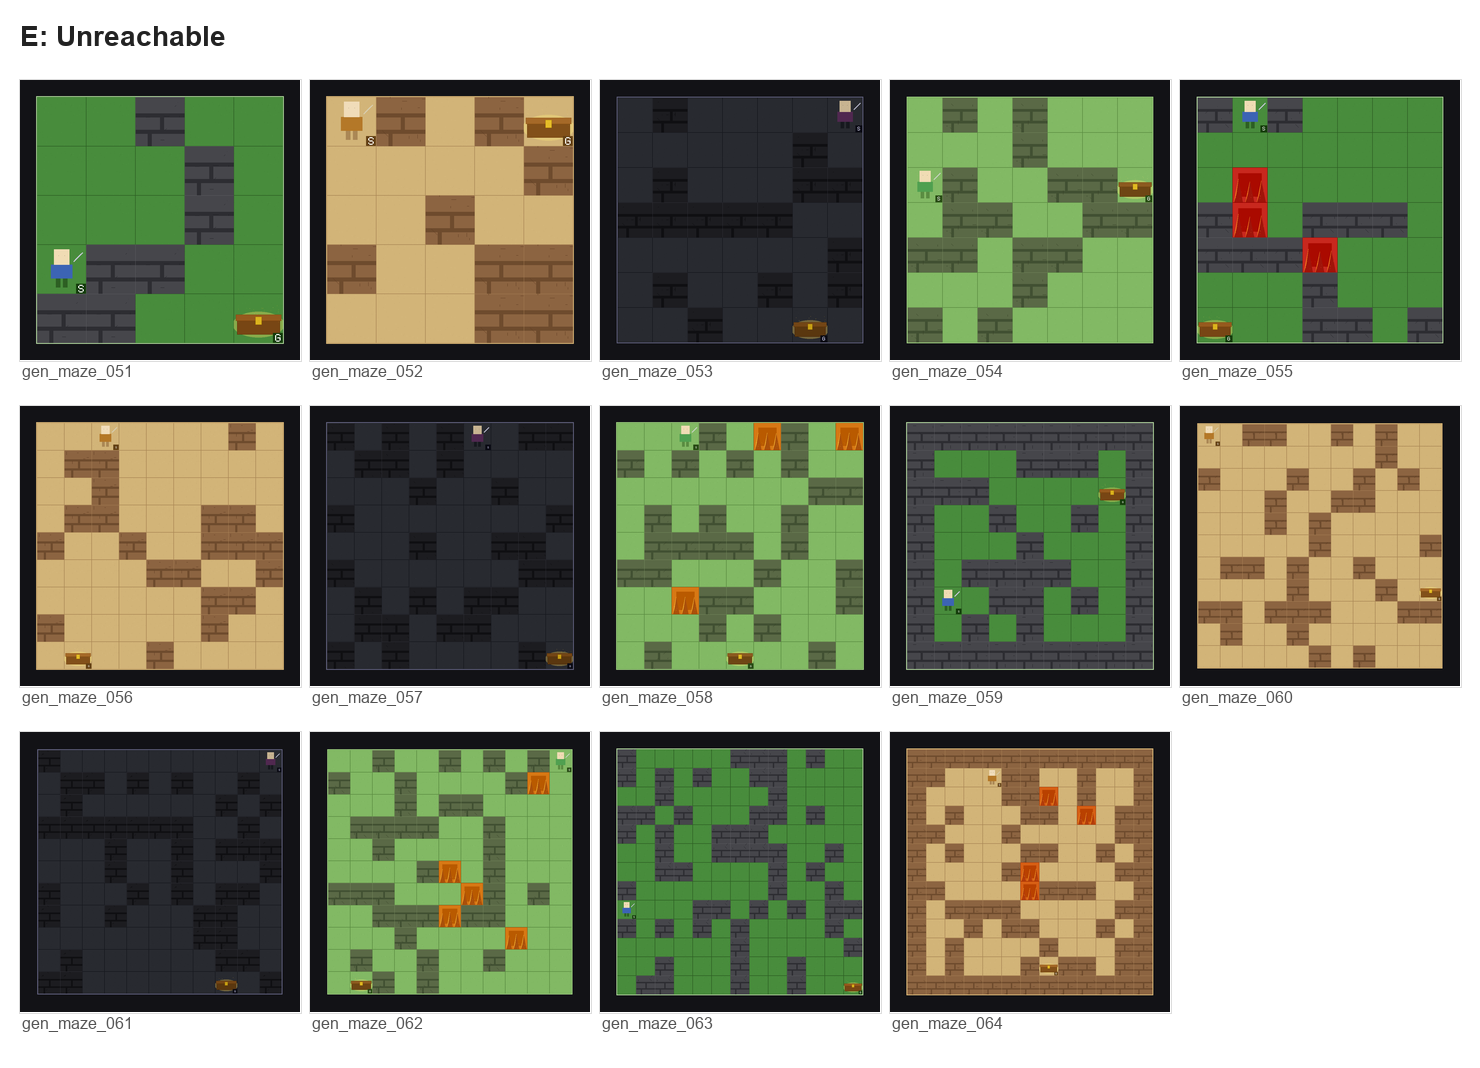
\includegraphics[width=0.85\textwidth]{appendix_group_e.png}
\caption{Group~E: Unreachable (14 mazes). All mazes have no valid path from start to goal.}
\label{fig:app_e}
\end{figure}

\begin{figure}[ht]
\centering
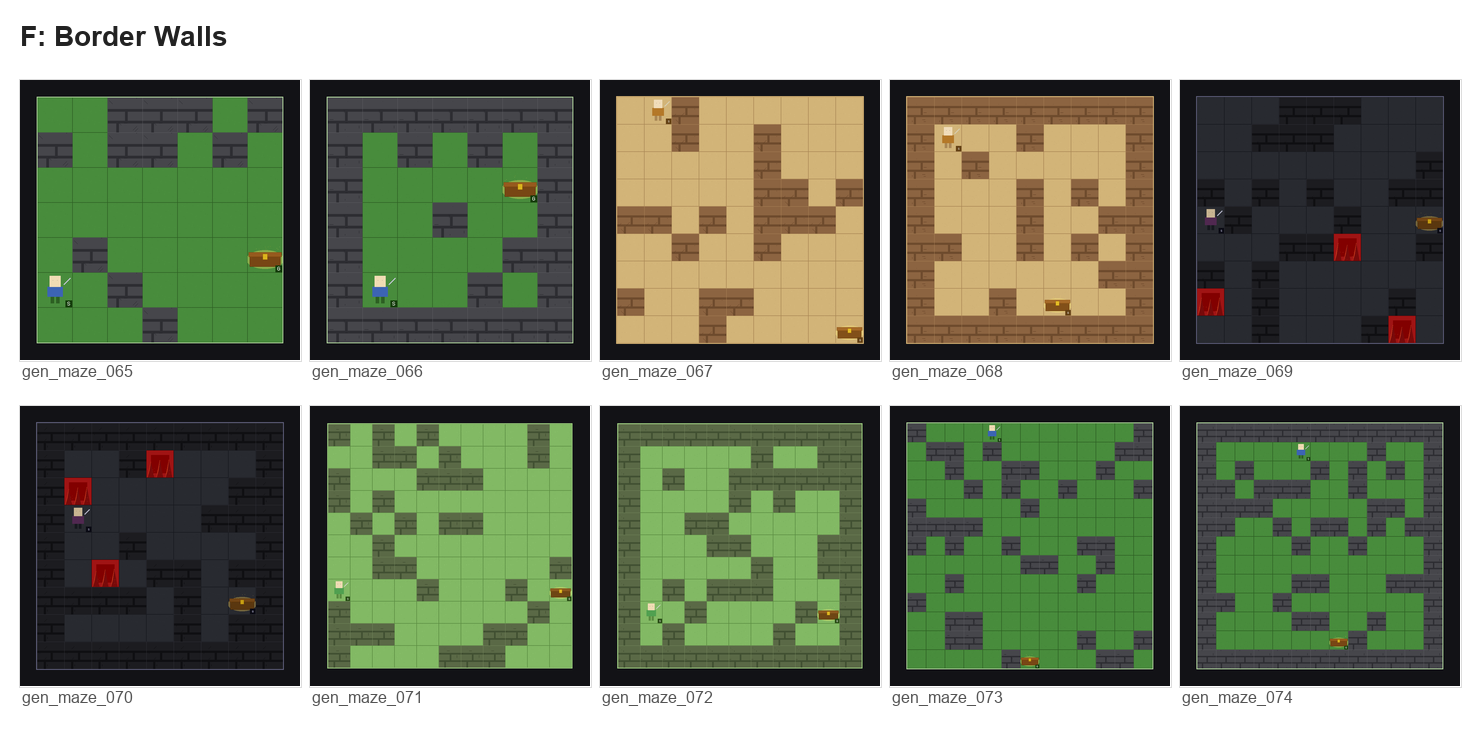
\includegraphics[width=0.85\textwidth]{appendix_group_f.png}
\caption{Group~F: Border Walls (10 mazes). Five matched pairs with and without a wall border ring.}
\label{fig:app_f}
\end{figure}

\begin{figure}[ht]
\centering
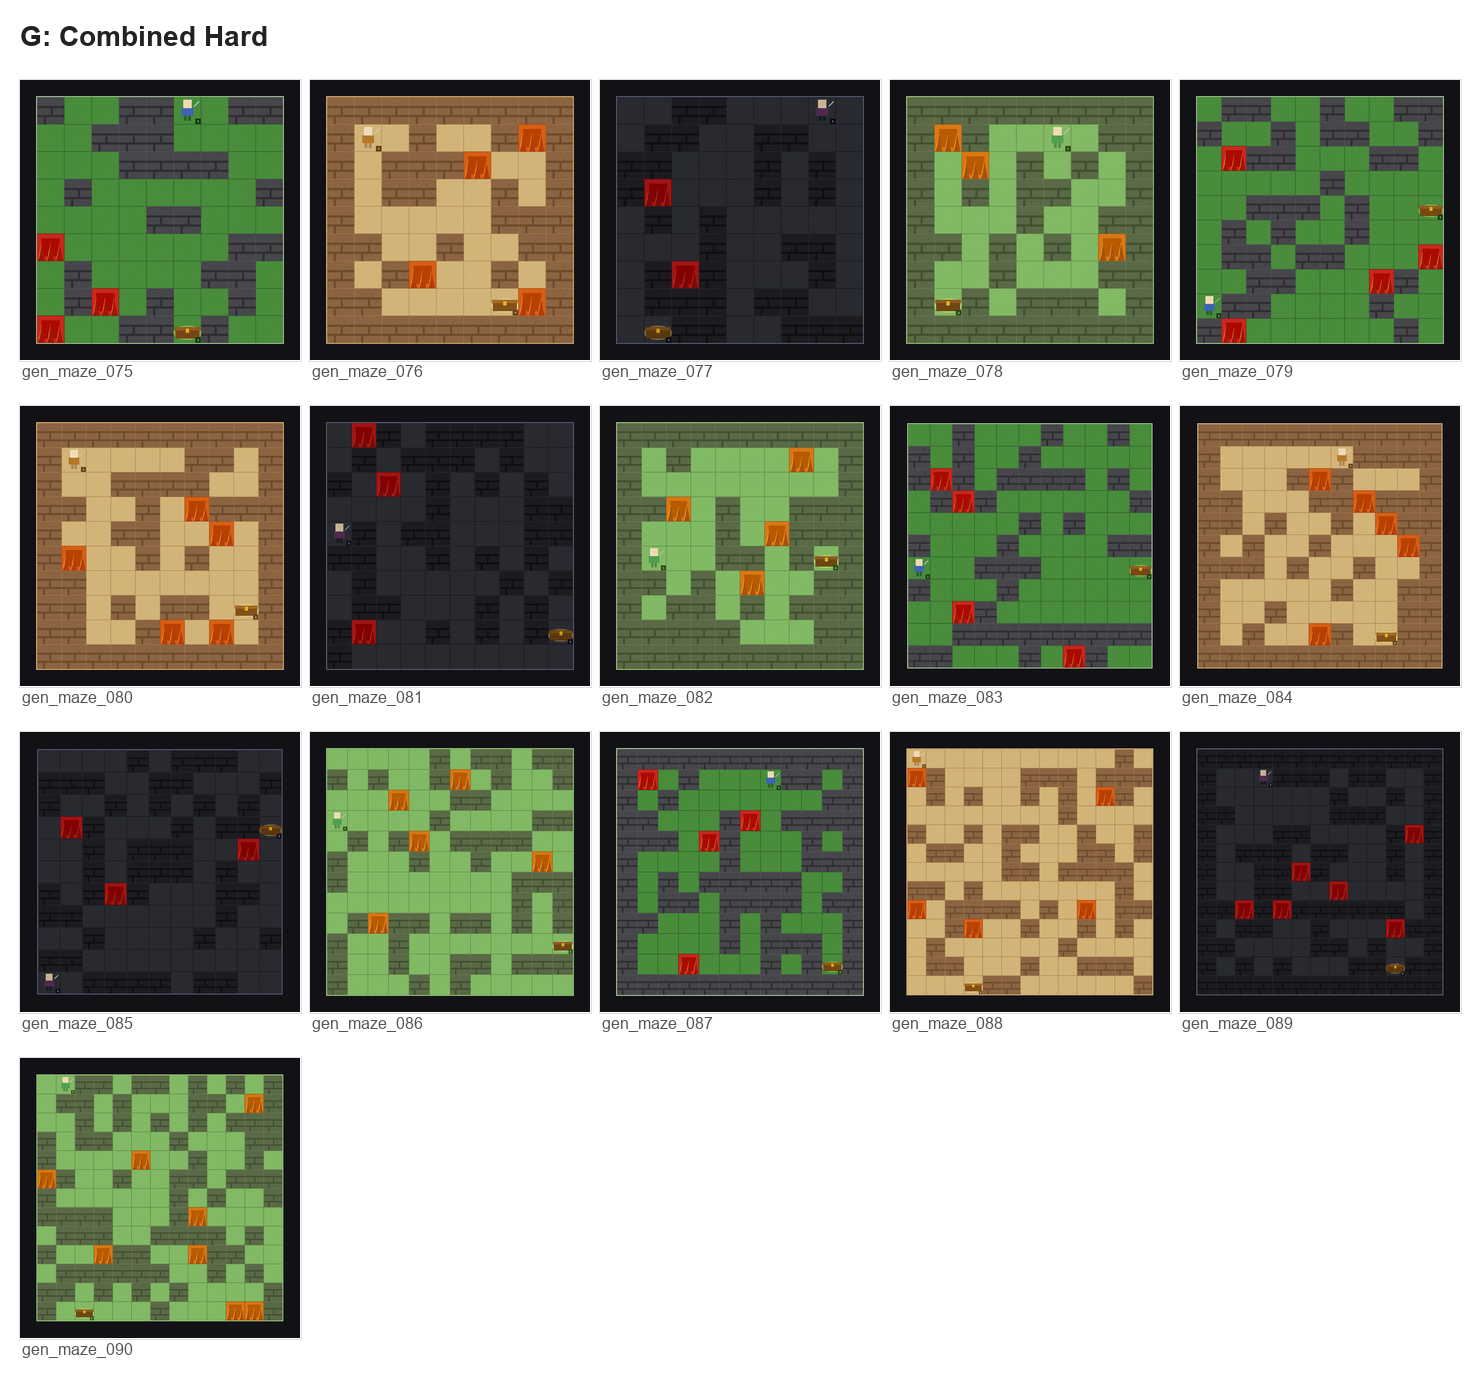
\includegraphics[width=0.85\textwidth]{appendix_group_g.png}
\caption{Group~G: Combined Hard (16 mazes). Large grids with high wall density, traps, and borders.}
\label{fig:app_g}
\end{figure}

\begin{figure}[ht]
\centering
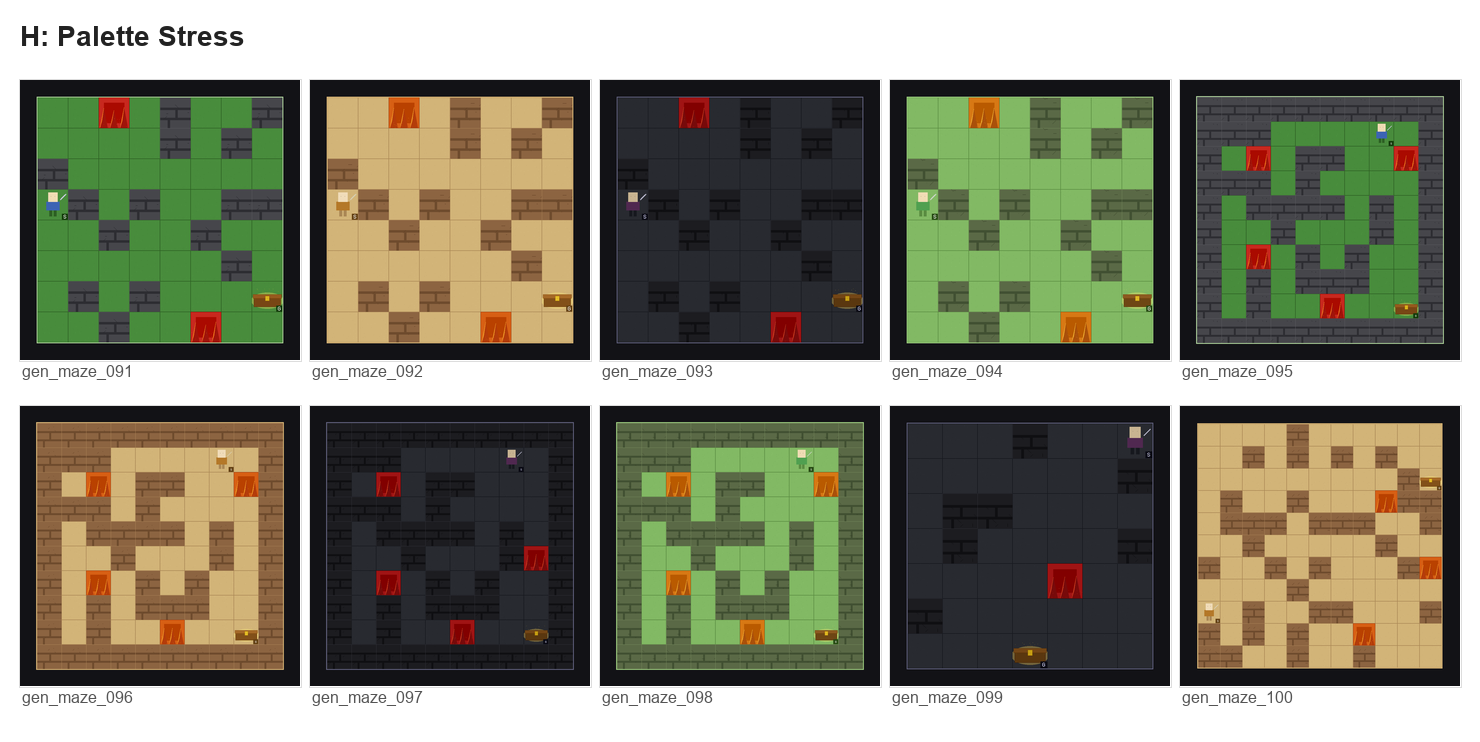
\includegraphics[width=0.85\textwidth]{appendix_group_h.png}
\caption{Group~H: Palette Stress (10 mazes). Same maze structure rendered across four visual palettes.}
\label{fig:app_h}
\end{figure}

\begin{figure}[ht]
\centering
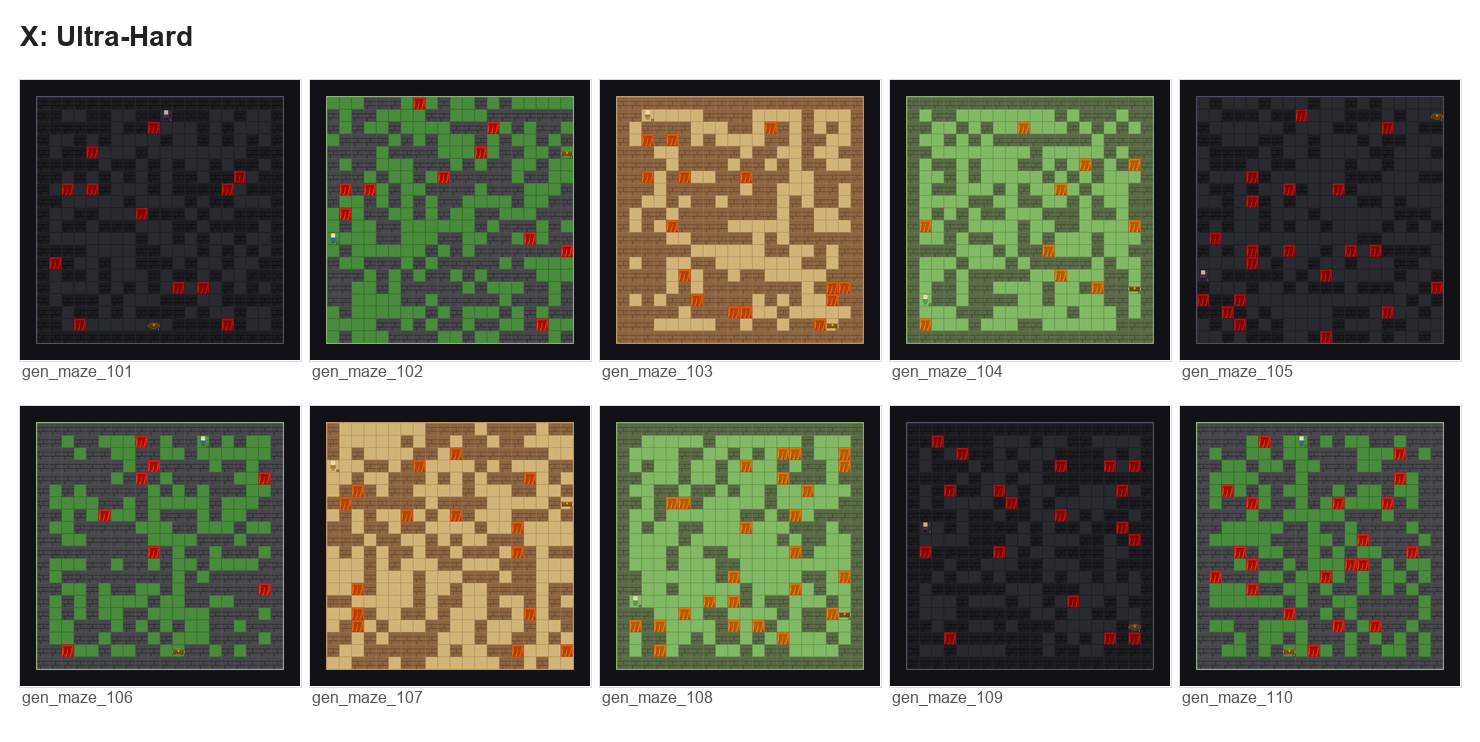
\includegraphics[width=0.85\textwidth]{appendix_group_x.png}
\caption{Group~X: Ultra-Hard (10 mazes). $20 \times 20$ grids with 8--25 traps and shortest paths of 28--42 steps.}
\label{fig:app_x}
\end{figure}

\end{document}
